\chapter{INTRODUCTION}\label{chap1}

\section{Music Recommendation System\cite{mainpaper}}
Recommender systems are techniques used for providing suggestion for a item related to various decision making process such as what items to buy or what music to listen.

These music recommendation systems are part of a broader class of recommender systems, which filter information to predict a user’s preferences when it comes to a certain item. There are mainly two  two classes, or approaches, to recommender systems ,Collaborative Filtering and Content Based Filtering.

\subsection{Content Based Filtering}
The content-based filtering approach used explicit features of the users and items. Content-based filtering closely examines the actual item to determine which features are most important in making recommendations and how those features interact with the user’s preferences. This approach need expertise in domain as we need to select features based on which recommendation can be made. Data collection can be much more complicated in content-based filtering as it is very difficult to select which features of an item will be important in creating some sort of predictive model.

\subsection{Collaborative Filtering}
Collaborative filtering relies only on past user behavior—for example,previous transactions or product ratings—without requiring the creation of explicit profiles. In this approach we either find the user to user closeness means based on various features we try to find other users which are most similar to user in question. And recommend items most liked by those other users. We may also find item to item closeness and using  previous liked item we can find items close to those(previous liked items) and recommend most close item. A major appeal of collaborative filtering is that its domain free which made it suitable to various task where finding explicit features are hard.

\begin{figure}
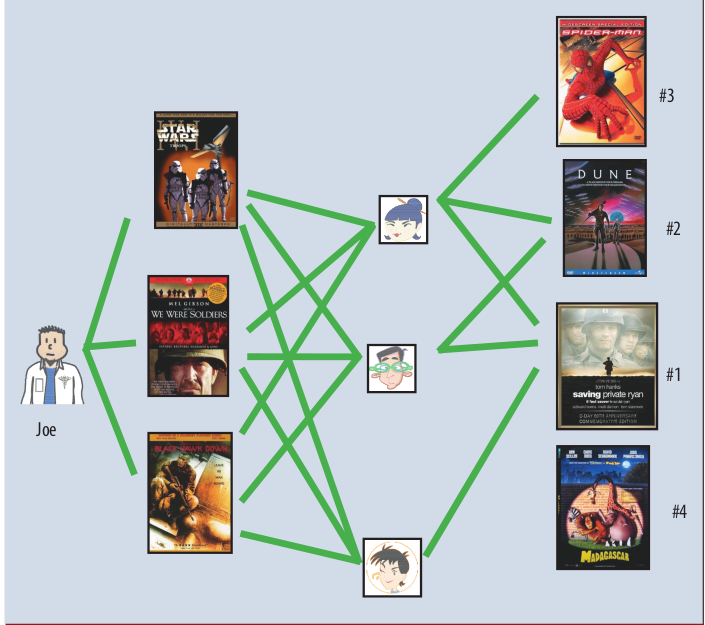
\includegraphics[scale=0.4]{colab}
\caption{Collaborative Filtering\cite{mainpaper}}
\label{chap0Fig:1}
\end{figure}

The user-oriented neighborhood method. Joe likes the three movies on the left. To make a prediction for him, the system finds similar and difficult to profile using content filter-users who also liked those movies, and then determines which other movies
ing. While generally more accurate than
they liked. In this case, all three liked Saving Private Ryan, so that is the first
content-based techniques, collaborative
recommendation. Two of them liked Dune, so that is next, and so on.


\subsection{Hybrid System\cite{hybrid}}
Hybrid systems means systems which are using both collaborative and content based filtering together. Hybrid systems are found to have better result than individual approaches alone.

\section{Music Playlist Generation} \label{sec1.1}
Music Playlist Generation simply means the task of generating a sequence of songs suitable for a particular user based on various inputs  given by the user. Inputs can be explicit like artist name, genre, current emotion or implicit like current time (users may like to listen to happy songs in morning) ,facial expression,etc. We have used artist name or band name as the input based on which playlist will be generated. 


\section{Music Playlist Shuffling} \label{sec1.1}
Music Playlist Shuffling means rearranging the playlist songs in such a order which is appealing to the user. It also mean changing the order dynamically based on user inputs(like whether user skipped current track or listened to the whole song or skipped in between)


